The structures that were initially box-shaped, with filter sizes 40 nm, 60 nm and 80 nm, respectively, are shown in Fig. \ref{fig:BoxStructures}, and  the initially Y-junction-shaped structures, also with filter sizes 40 nm, 60 nm and 80 nm, respectively, are shown in Fig. \ref{fig:Y-juncStructures}. As mentioned in the "Filter size" subsection, we see that the designs are not without shaded areas. This is especially true for the structures with larger filter sizes. \\

\subsection{Fabricating the designs}
The fabrication is executed using spin coating, resists, electron beam lithography (e-beam), chemical vapor deposition (CVD), and etching. The designs were fabricated by Lars Hagedorn Frandsen from DTU Photonics \cite{Fabrication}. Since the e-beam removes material from top to bottom chronically, it is not possible to fabricate homogeneous columns of specific concentration of Si and air without a very advanced O$_2$ doping process. Therefore the shaded areas must be converted to black and white, and consequently treated binarily as silicon or air.\\

This is done with a threshold value for silicon concentration, deciding if the area is set to silicon or air. Since the shaded areas are important to the efficiency of the design, forcing the the shaded area into either black or white will sadly lead to a downgrade in performance. The minimum possible feature sizes written with e-beam is around 20 nm \cite{DanchipOfficial}, making it is possible to fabricate structures with a filter size of 40 nm. As seen in Fig. \ref{fig:BoxStructures}, the fabricated structures with feature size 40 nm were remarkably close to the simulated structures.

\newpage

 \subsection{Box structures}

 \begin{figure}[H]
    \centering
    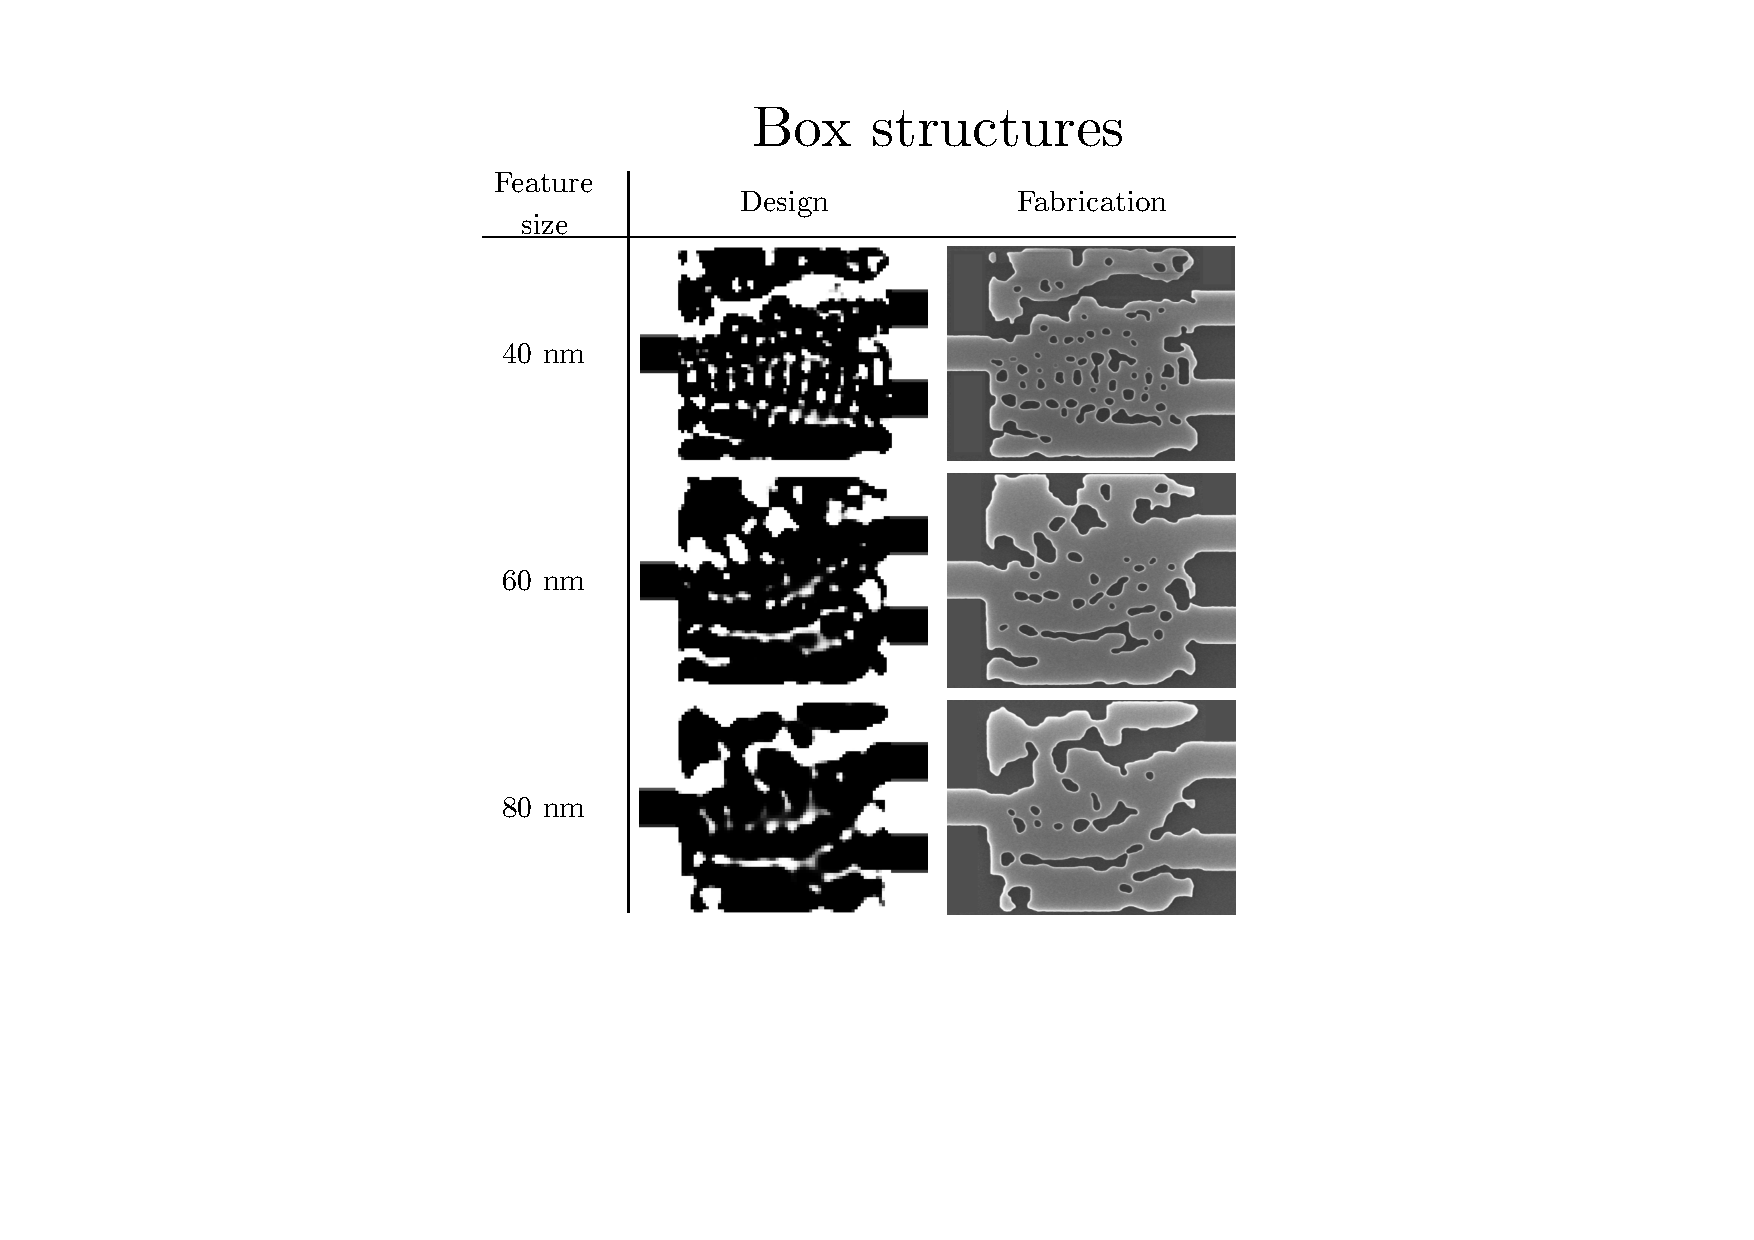
\includegraphics[trim= 8.35cm 2.73cm 8.35cm 2.73cm,clip,width=\textwidth]{fig/boxstructures.pdf}
    \vspace{-2cm}
    \caption{Box structures. Fabrication flaws are evident across all feature sizes, although one would expect the small feature sizes to have more errors due to the higher precision needed. This is due to the fact that a larger feature size also have larger shaded regions, which were not possible to fabricate with our fabrication process. PhaZor uses shaded (grey) pixels to represent materials with property values between silicium and air. In each iteration step, less shading is permitted. When fabricating the structures shown to the left, the coloring is converted to binary: material is either removed (black) or kept (white).}
    \label{fig:BoxStructures}
 \end{figure}

 \newpage
 \subsection{Y-junction structures}
 \begin{figure}[H]
    \centering
    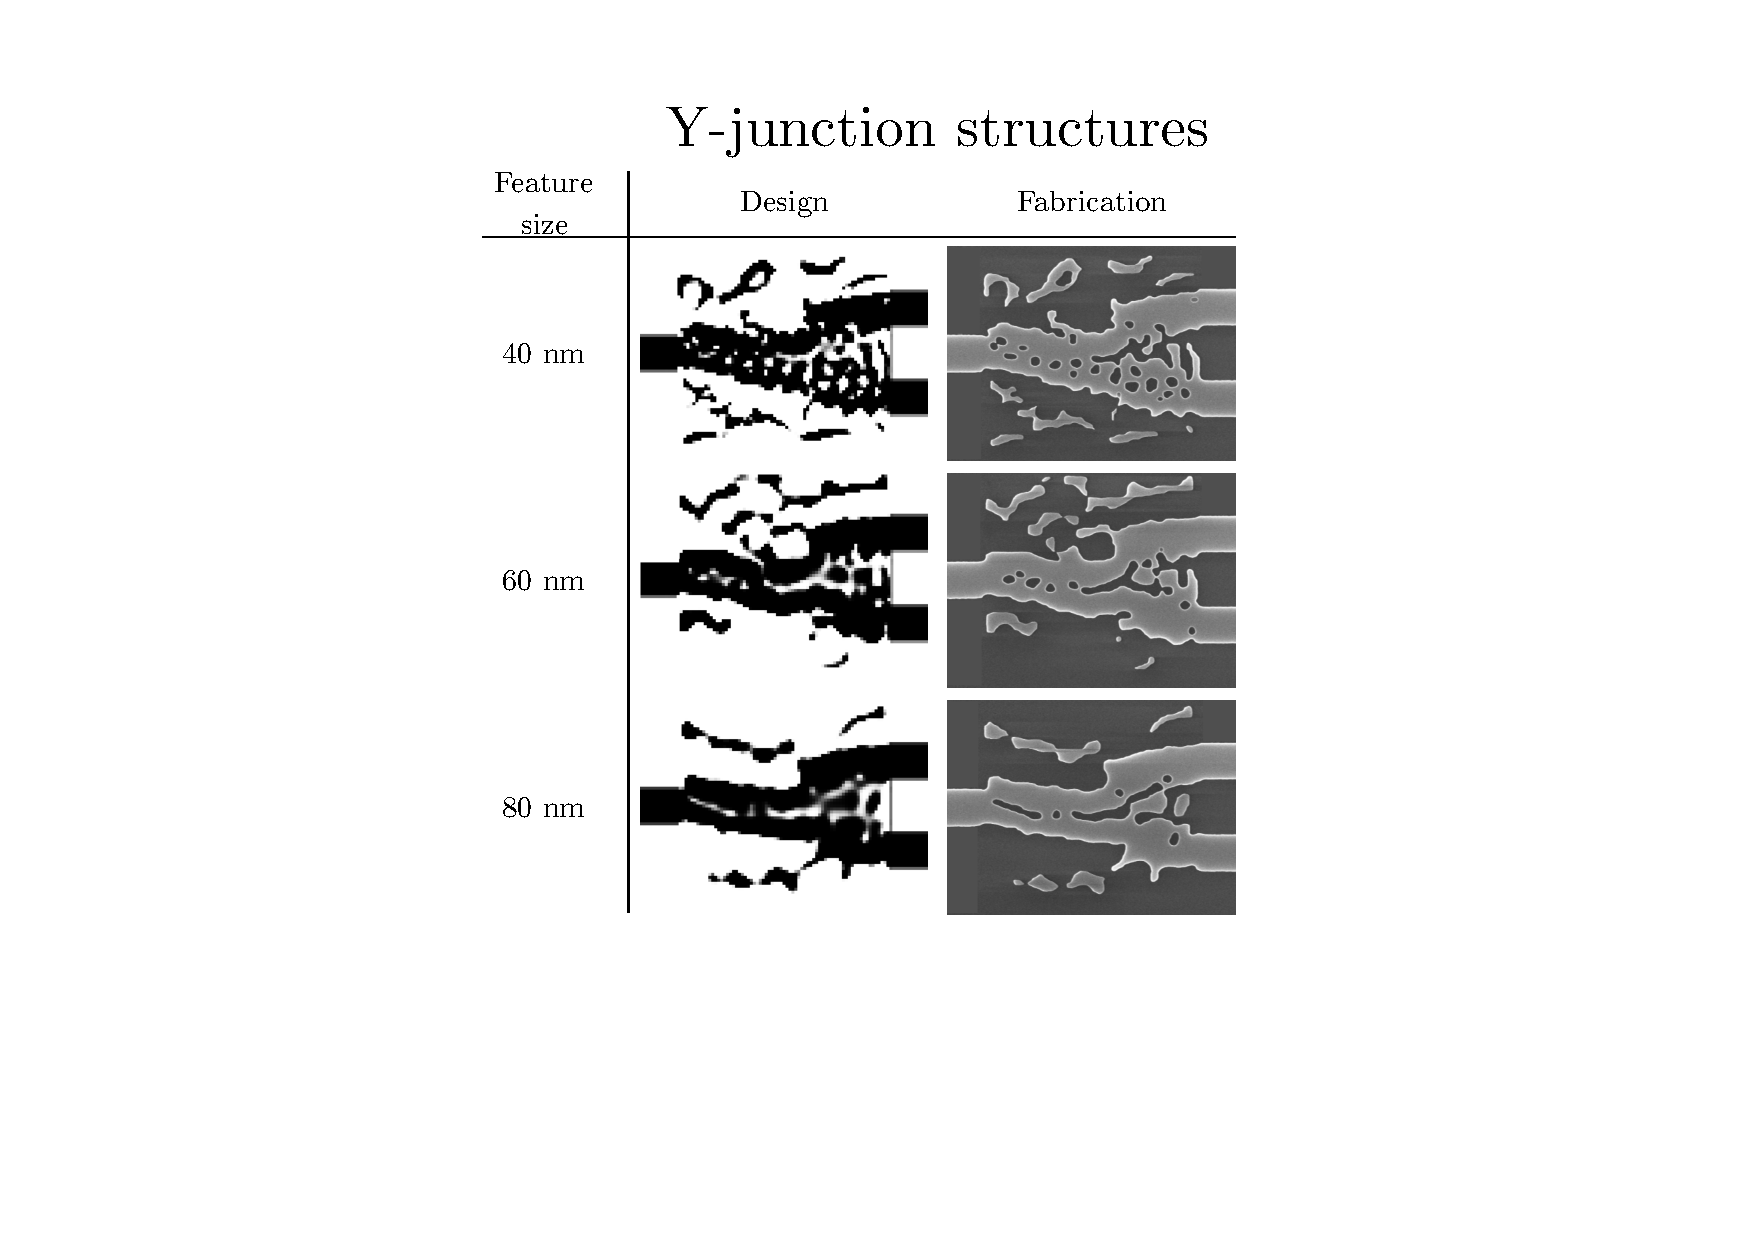
\includegraphics[trim= 8.35cm 2.73cm 8.35cm 2.73cm,clip,width=\textwidth]{fig/yjunctionstructures.pdf}
        \vspace{-2cm}
    \caption{Y-junction structures. Fabrication flaws are evident across all feature sizes, although one would expect the small feature sizes to have more errors due to the higher precision needed. This is due to the fact that a larger feature size also have larger shaded regions, which were not possible to fabricate with our fabrication process. PhaZor uses shaded (grey) pixels to represent materials with property values between silicium and air. In each iteration step, less shading is permitted. When fabricating the structures shown to the left, the coloring is converted to binary: material is either removed (black) or kept (white). PhaZor added material in the initially material-void regions, so the outer edges of the structure no longer outline (simple) Y-junctions.}
    \label{fig:Y-juncStructures}
\end{figure}

 \newpage